\chapter{Atoms in Magnetic Field}

\section{Magnetic Moment of Atoms}

\begin{equation*}
  \begin{aligned}
    \mu_L = - \dfrac{e}{2m}p_l = - \sqrt{l \left( l + 1 \right)} \mu_B
    \quad\quad
    \quad\quad
    \quad\quad
    \mu_B = \dfrac{e h}{2 \pi m} = \dfrac{e\hbar}{2m}   
    \quad
    \text{(Bohr magneton)}
  \end{aligned}
\end{equation*}

\section{Lande Factor}

\begin{equation*}
  \begin{aligned}
    g = 1 + \dfrac{j \left( j + 1 \right) - l \left( l + 1 \right) + s \left( s + 1 \right)}{2 j \left( j + 1 \right)} 
  \end{aligned}
\end{equation*}

For single electron atom:

\begin{equation*}
  \begin{aligned}
    \mu_j = g \dfrac{e}{2m} p_j 
  \end{aligned}
\end{equation*}

For multi electron atom:

\begin{equation*}
  \begin{aligned}
    \mu_J = - g \dfrac{e}{2m} P_J 
  \end{aligned}
\end{equation*}

\section{Energy of Atom in Magnetic Field}

\begin{figure}[H]
  \centering
  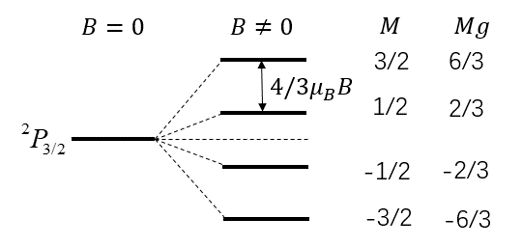
\includegraphics[width=0.7\linewidth]{figures/energy-magnetic.png}
\end{figure}

\begin{equation*}
  \begin{aligned}
    \Delta E = \left( M_2 g_2 - M_1 g_1 \right) \mu_B B 
    \quad\quad 
    \quad\quad 
    M = J,J-1,J-2,\dots,-J
  \end{aligned}
\end{equation*}

\begin{equation*}
  \begin{aligned}
    \Delta \tilde{\nu} = \dfrac{1}{\lambda'} - \dfrac{1}{\lambda} = \left[ M_2 g_2 - M_1 g_1\right] \dfrac{Be}{4 \pi m c} = \left[ M_2 g_2 - M_1 g_1 \right] L
    \quad\quad
    \quad\quad
    L = \dfrac{Be}{4 \pi m c} 
  \end{aligned}
\end{equation*}

\begin{figure}[H]
  \centering
  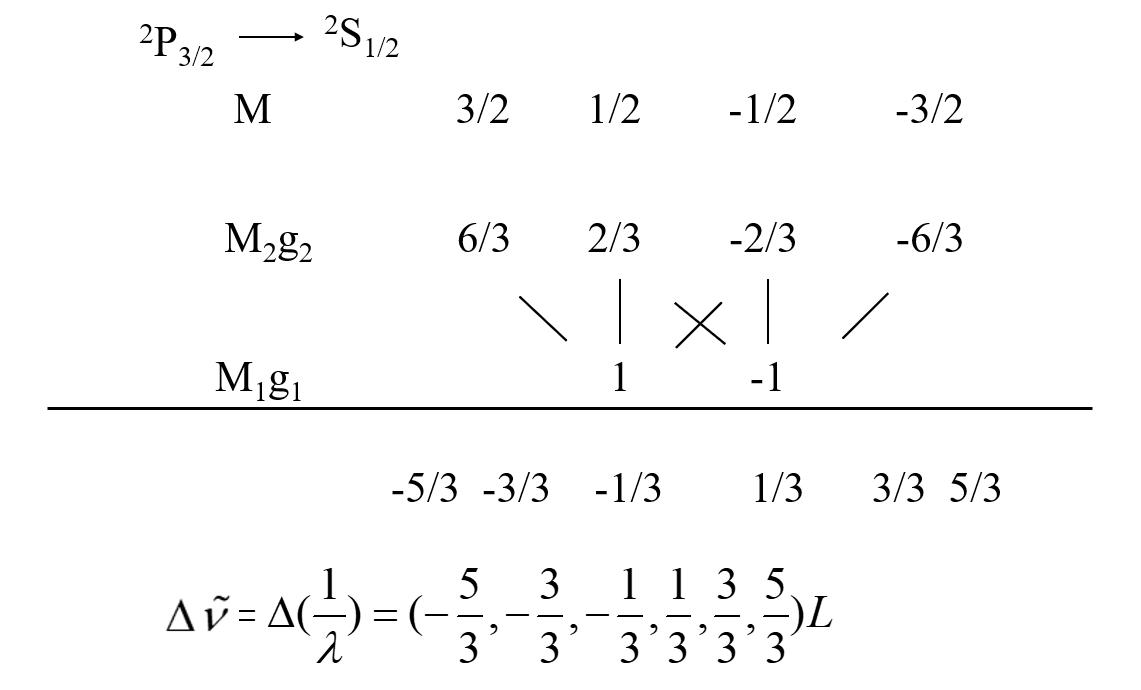
\includegraphics[width=0.7\linewidth]{figures/energy-magnetic-2.png}
\end{figure}

\section{Selection Rule}

\begin{equation*}
  \begin{aligned}
    \Delta M = 0 \quad \Rightarrow \quad \pi \\
    \Delta M = \pm 1 \quad \Rightarrow \quad \sigma
  \end{aligned}
\end{equation*}

$\pi$ beam cannot be observed in the perspective which is parallel to $B$, both beam can be observed in the perspective perpendicular to $B$.

\section{Abnormal Zeeman effect}

\begin{equation*}
  \begin{aligned}
    \Delta \tilde{\nu} = \left[ M_2 g_2 - M_1 g_1 \right] L \neq \pm L
    \quad \Rightarrow \quad
    M_2 g_2 - M_1 g_1 \neq \pm 1
  \end{aligned}
\end{equation*}

%%% Local Variables:
%%% mode: latex
%%% TeX-master: "Atomic_Physics"
%%% End:
